\chapter{Konzeptuelle Grundlagen und verwendete Datenstrukturen}
\label{chapter:grundlagen}

\section{Konzeptuelle Grundlagen}

Dieser Abschnitt beschreibt die wesentlichen konzeptuellen Grundlagen, die in dieser Arbeit an mehreren Stellen verwendet werden und daher an zentraler Stelle erläutert werden.

\subsection{Die unterliegende Datenstruktur des Pose-Graphen}
\label{section:pose_graph}

Die Grundlage für den in dieser Arbeit vorgeschlagenen Ansatz bietet die Implementation einer Datenstruktur für den Pose-Graphen, im Folgenden auch Pose-Historie oder Pfad genannt. Die Datenstruktur ist dabei einfach aufgebaut. Sie hält einen indizierten Vektor aus Posen $\left\lbrace P_0, ..., P_n \right\rbrace$ und kapselt die Funktionalität für das Einfügen dieser Posen. Zusätzlich ist in der Datenstruktur die Funktionalität zur Identifikation von Schleifenschluss-Kandidaten gespeichert.

\subsection{Koordinatensysteme}

Ein wesentliches Konzept bei der Verarbeitung räumlicher Daten ist die Verwendung von Koordinatensystemen.
Sie werden genutzt um die Positionen von Daten und Objekten im Raum zu beschreiben.
Koordinatensysteme können für sich alleine stehen oder relativ zu anderen Koordinatensystemen.
Im Dreidimensionalen besitzt ein Koordinatensystem drei verschiedene Achsen (x, y und z-Achse), die jeweils im 90 Grad Winkel zueinander ausgerichtet sind.
Rotationen im Raum werden beschrieben als Rotationen um die jeweiligen Achsen.
Welche Achse in welche Richtung zeigt ist nicht eindeutig definiert.
Es gibt jedoch verschiedene Standards beziehungsweise Konventionen wie das links- oder rechtshändische Koordinatensystem.
In ROS wird konventionell ein rechtshändisches Koordinatensystem, abgebildet in Abbildung \ref{fig:ros_coordinate_sys} dargestellt. Dies wird im Folgenden ebenfalls als Standard verwendet.

\begin{figure}
		\centering
		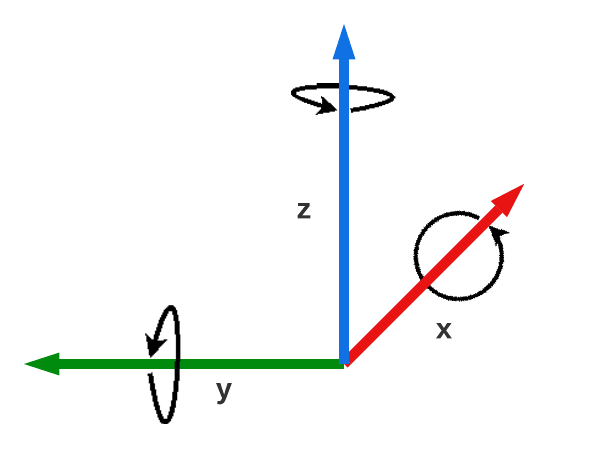
\includegraphics
			[scale=0.25]
			{ros_coordinate_sys}
		\caption
			[Caption for LOF]{Schematische Darstellung der Konvention für Koordinatensysteme im ROS Framework. Die z-Achse zeigt nach oben, die x-Achse nach vorne und die y-Achse nach links. Die Rotation um die Achsen ist entsprechend der Konvention im Uhrzeigersinn.}			                                                                                                                                     
		\label{fig:ros_coordinate_sys}
	\end{figure}

In der Robotik kommt es häufig vor, dass verschiedene (bewegliche) Komponenten relativ zu einem globalen Bezugssystem oder relativ zueinander beschrieben werden müssen. Die Bewegung eines übergeordneten Bezugssystems kann implizit für eine Veränderung der relativ zu diesem Bezugssystem platzierten Systeme führen.
Dies lässt sich anhand eines Arm-Roboters zeigen, der mehrere miteinander verbundene Gelenke hat. Bewegt sich ein Gelenk werden automatisch auch die am Arm weiter außen befindlichen Gelenke mitbewegt. Aus Sicht des bewegten, übergordneten Bezugssystems hat sich die Position der untergeordneten Gelenke nicht verändert, aus Sicht des globalen Bezugssystems, wie zum Beispiel dem Montierungspunkt des Roboters, allerdings schon.

In ROS werden Anhängigkeiten zwischen Bezugssystemen in einer Baumstruktur, genannt \textit{transformation tree (tf-tree)} dargestellt.
Die Wurzel dieser Baumstruktur ist das globale Bezugssystem, wie zum Beispiel der Ursprung einer globalen Karte oder der Startpunkt der Trajektorie eines Roboters.
Das globale Bezugssystem kann beliebig gewählt werden.
Auf diese Weise kann ein Koordinatensystem, welches relativ zu einem anderen gelegen ist im Baum als Kindknoten seinem Bezugssystem untergeordnet werden. Es wird nur die relative Transformation (s. Kapitel \ref{section:transformationen}) zwischen den Systemen im Baum gespeichert.
Dies hat den Vorteil, dass bei der Bewegung eines Systems die untergordneten Systeme nicht ebenfalls verändert werden müssen, da deren Transformationen relativ zum bewegten Bezugssystem angegeben sind und nicht global zur Wurzel des Baumes.
Abbildung \ref{fig:robot_tf} zeigt ein Beispiel für einen Roboter mit mehreren voneinander abhängigen System.


\begin{figure}
		\centering
		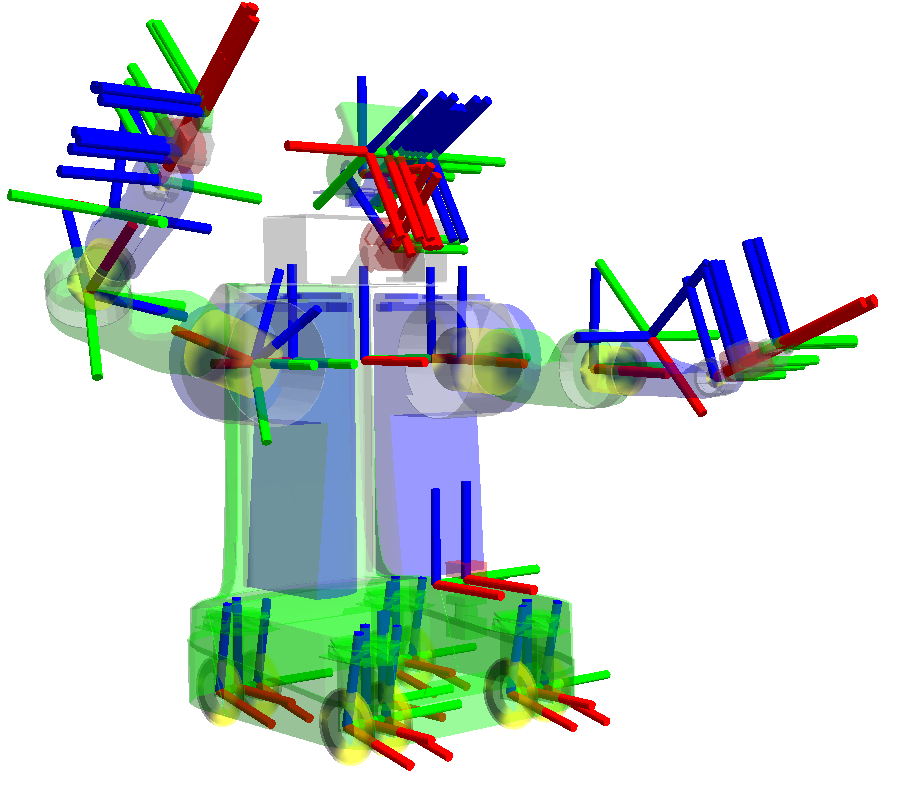
\includegraphics
			[scale=0.28]
			{robot_tf}
		\caption
			[Caption for LOF]{Schematische Darstellung eines Roboters und dessen beweglicher Teile. Die Ausrichtung der jeweiligen Gelenke wird mit einem lokalen Koordinatensystem beschrieben. Die globale Position einzelner Teile kann durch eine Verkettung der relativen Transformation in Richtung der Wurzel des Baumes bestimmt werden.
			Bild aus: \cite{ros_tf_image}}			                                                                                                                                     
		\label{fig:robot_tf}
	\end{figure}

Auch räumliche Daten wie zum Beispiel Punktenwolken aus Laserscannern können relativ zu verschiedenen Koordinatensystemen gesehen werden.
So kann es nützlich sein die Punktwolke relativ zum Koordinatensystem des Scanners oder innerhalb des globalen Koordinatensystems zu betrachten. Um zwischen den Koordinatensystemen zu wechseln wird eine Koordinatensystemtransormation. Diese werden im folgenden Kapitel behandelt.

 
\subsubsection{Transformationen}
\label{section:transformationen}

Eine Koordinatensystemtransformation ist ein Sonderfall einer mathematischen Transformation, die eine Menge $X$ auf sich selbst abbildet:
\begin{myequation}
f: X \rightarrow X
\end{myequation}

Eine Koordinatensystemtransformation beschreibt die Differenz zwischen zwei unterschiedlichen Koordinatensystemen und enthält sowohl die Translationsdifferenz als auch die Rotationsdifferenz.
Zur Berechnung dieser Transformation zwischen zwei beliebigen Koordinatensystem $C_1$ und $C_2$ wird die absolute Translation und Rotation beider Koordinatensysteme zum Ursrungskoordinatensystem, wie zum Beispiel den Urpsrung einer Umgebungskarte, benötigt.
Durch diese Rotations und Translationskomponenten beschreibt sich die absolute Position und Rotation der Koordinatensysteme im Raum aus Sicht des Ursprungskoordinatensystems $C_{MAP}$. Diese absolute Position und Rotation ist die Transformation von den jeweiligen Koordinatensystemen ins Urpsrungskoordinatensystem.

Es existieren diverse Darstellungsweisen für Koodinatensystemtransformationen. Eine mögliche Darstellung ist die als Vektor. In folgendem ist die Transformation vom Koordinatensystem $C_X$ ins Koordinatensystem $C_{MAP}$ dargestellt. Die Variablen $t_i$ bezeichnen dabei die Translationskomponenten und die Variablen $r_i$ die Rotationskomponenten um die jeweiligen Achsen. 

\begin{myequation}
T_{C_X \rightarrow C_{MAP}} = \left( t_x,t_y,t_z,r_x,r_y,r_z \right)^T
\end{myequation}

Neben der Vektordarstellung kann eine Transformation zusätzlich als eine $4x4$ Matrix dargstellt werden.
Diese Darstellungsweise hat den Vorteil, dass die Transformation direkt per Matrixmultiplikation auf Daten wie um homogene Koordinaten erweiterte Punktdaten angewandt werden kann.
Auch die direkt Kombination verschiedener Transformationen ist durch eine Matrixmultiplikation möglich. Hier gilt es zu beachten, dass Matrixmultiplikation nicht kommutativ ist und ein Vertauschen der Reihenfolge bei der Multiplikation zu unterschiedlichen Ergebnissen führen kann.
Bei einer Verkettung von Transformationen durch Multiplikation wird die Matrix zuerst angewandt, welche am Ende der Multiplikation steht.

In dieser Arbeit werden Transformationen zum Beispiel verwendet um zu bestimmen, wie sich ein Roboter zwischen zwei Messungen bewegt hat. Diese Transformationen beschreiben relative Differenzen zwischen Roboterpositionen im Raum. Diese Roboterpositionen werden auch \emph{Posen} genannt.
Eine Pose ist dabei eine meist absolute Beschreibung der Translation und Rotation eines Roboters zu einem gewissen Zeitpunkt $t$ aus Sicht des Ursprungskoordinatensystems wie zum Beispiel dem Karten-Ursprung $C_{MAP}$.


\begin{figure}
		\centering
		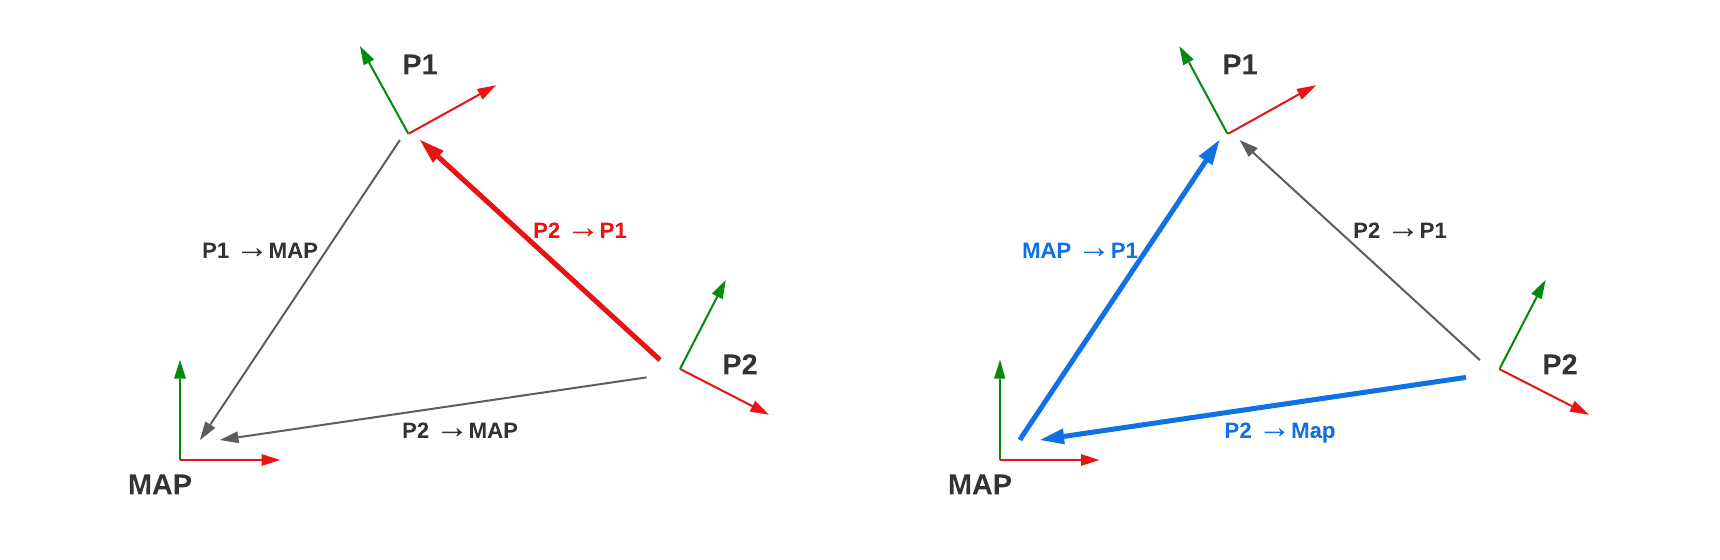
\includegraphics
			[scale=0.25]
			{transformation}
		\caption
			[Caption for LOF]{Schematische Darstellung der bestimmung einer Transformation zwischen zwei Roboter-Posen $P_1$ und $P_2$, hier zur Vereinfachung dargestellt in 2D. Gesucht ist die Transformation $\left( T_{P_2 \rightarrow P_1} \right)$, dargestellt im linken Teil der Abbildung als roter Pfeil. Diese kann implizit bestimmt werden durch eine Verkettung der Transformationen $T_{P_2 \rightarrow MAP}$ und $T_{MAP \rightarrow P1}$, hier dargestellt im rechten Teil der Abbildung in blau. Die Transformation $T_{MAP \rightarrow P1}$ ist dabei nicht explizit gegeben. Sie kann berechnet werden durch eine Inversion der Transformation $T_{P1 \rightarrow MAP}$. Die finale Gleichung zur Berechnung der relativen Transformation ist dargestellt in Gleichung \ref{equation:transformation}.}			                                                                                                                                     
		\label{fig:transformation}
	\end{figure}


Abbildung \ref{fig:transformation} zeigt die Mathematik hinter der Berechnung der Posedifferenz exemplarisch. Es wird deutlich, dass eine gesuchte Transformation aus dem Koordinatensystem von Pose $P_2$ in das Koordinatensystem von Pose $P_1$  $\left( T_{P_2 \rightarrow P_1} \right)$ gegeben ist durch:

\begin{myequation}
\label{equation:transformation}
\left( T_{P_2 \rightarrow P_1} \right) = \left(T_{P_1 \rightarrow MAP} \right)^{-1} * T_{P_2 \rightarrow MAP}
\end{myequation}

Basierend auf den erläuterten mathematischen Grundlagen wird in Kapitel \ref{section:slam} die Grundlagen von SLAM, insbesondere von TSDF basierten SLAM Verfahren, erörtert.
Zuvor werden in nachfolgendem Abschnitt die Eigenschaften und Anwendungsbereiche der TSDF beschrieben.

\section{TSDF}
\label{section:tsdf}

Zur Lösung des \emph{Simulatneous Localization and Mapping (SLAM)} (siehe Kapitel \ref{section:slam}) Problems in unbekannten Umgebungen wird im Regelfall eine Form der Kartenrepräsentation und die Algorithmik benötigt, sich auf Basis der Kartenrepräsentation zu lokalisieren um diese im Anschluss aktualisieren zu können. Bei vielen Lösungsansätzen wie zum Beispiel einer inkrementellen \emph{Registrierung (siehe Kapitel \ref{section:slam})} mit dem \emph{Iterative Closest Point (ICP)} \cite{Besl:1992} oder \emph{Generalized Iterative Closest Point} \cite{segal2009generalized} Algorithmus werden als Kartenrepräsentation registrierte Punktwolken verwendet. Punktwolken stellen dabei keine geschlossenen Oberflächenrepräsentationen dar und benötigen viel Speicher im Gegensatz zu einigen geschlossenen Repräsentationen wie aus den Punktwolken generierten Dreiecksnetzen. Ein großer Nutzen einer solchen Repräsentation ist die vereinfachte Lokalisierung und Navigation auf Basis der Kartenrepräsentation durch deren Geschlossenheit beziehungsweise Kontinuität. Eine weitere Form der geschlossenen Oberflächenrepräsentation der Umgebung sind \emph{Signed Distance Fields (SDF)}. Im Gegensatz zu Dreiecksnetzen sind die SDF implizite, volumetrische Beschreibung der Oberfläche \cite{werner2014truncated}. Sie beschreiben die Oberfläche nicht direkt, sondern den Raum um die Oberfläche herum. Die \emph{Signed Distance} ist die orthogonale metrische Distanz eines beliebigen Punktes $p$ zur Oberfläche räumlicher Daten, wie zum Beispiel der approximierten Oberfläche von Punktwolken. Diese Distanz kann sowohl negativ, als auch positiv sein. Unterschieden wird zwischen dem Innenbereich, räumlich gesehen vor einer Wand oder einem Hindernis, und dem Außenbereich, welcher räumlich gesehen hinter dem vom Laser getroffenen Objekt befindlich ist. Positive SDF-Werte kennzeichnen Freiraum, negative den Raum hinter gesehenen Oberflächen oder Hindernissen. Der Übergang zwischen positiven und negativen TSDF-Werten beschreibt näherungsweise die gesehene Oberfläche.
Abbildung \ref{fig:tsdf} zeigt ein schematisches Beispiel für eine zweidimensionale, diskretisierte TSDF nach Abtasten der Oberfläche einer unbekannten Umgebung durch einen Laserscanner.

\begin{figure}
		\centering
		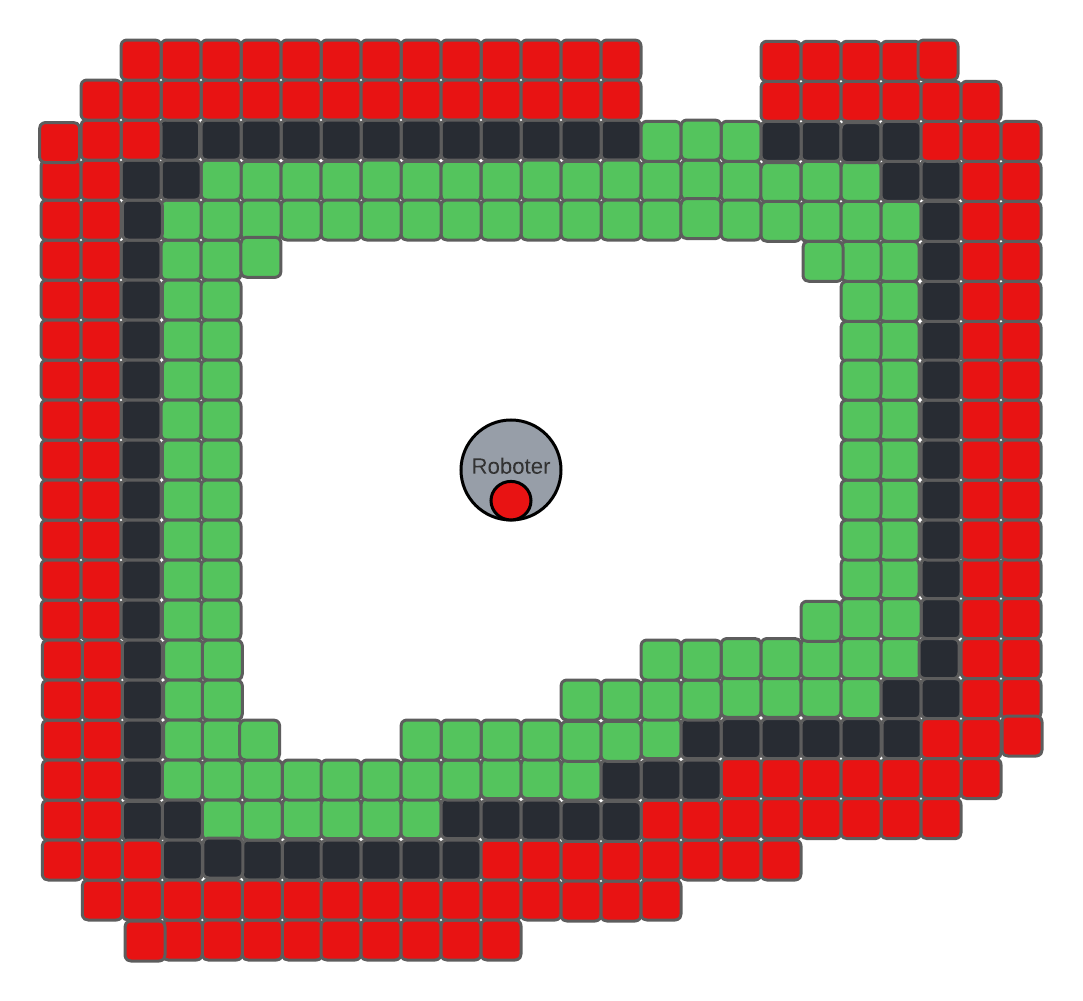
\includegraphics
			[scale=0.22]
			{TSDF}
		\caption
			[Caption for LOF]{Schematische Darstellung einer diskretisierten 2-D TSDF Karte. Abgebildet sind nur Voxel mit TSDF-Werten im Intervall $ \left] -\tau, \tau \right[$. In der Mitte der Karte befindet sich ein Roboter mit einem Laserscanner (hier dargestellt in rot). Der Roboter befindet sich zum Beispiel in einem Raum. Der Innenbereich (des Raumes) mit positiven TSDF-Werten ist hier dargestellt in grün, der Außenbereich mit negativen TSDF-Werten in rot. Die Oberfläche, in deren Umgebung die TSDF-Werte nahezu Null sind, ist abgebildet in schwarz.}			                                                                                                                                     
		\label{fig:tsdf}
\end{figure}

Die \emph{Truncated Signed Distance Funtion (TSDF)} ist eine Unterklasse der SDF. Sie betrachtet die Distanz zur Oberfläche nur bis zu einer maximalen Distanz $tsdf_{max}$, auch $tau \left(\tau)\right)$ gennant\cite{HATSDF}. Alle Werte die weiter von der Oberfläche entfernt oder unbekannt sind, erhalten als Wert $tau$ selbst. Dies spart Rechenaufwand, da nur die Werte in direkter Nähe zur Oberfläche angepasst werden müssen. In Gebieten, in denen der TSDF-Wert $tau$ entspricht, kann jedoch keine Aussage darüber getroffen werden, wo die nächste Oberfläche ist, oder wie weit sie entfernt ist. Es ist lediglich bekannt, dass die betrachtete Position nicht in direkter Nähe zur Oberfläche befindlich und mindestens $tau$ entfernt ist. Das Intervall möglicher Werte $\upsilon_i$ der TSDF ist:

\begin{myequation}
I_{\upsilon} = [-\tau, \tau]:= \lbrace x \in \mathbb{R} \rvert \tau > 0 \rbrace
\end{myequation}


Über SDF und TSDF können kontinuierliche Karten erstellt werden. Da kontinuierliche Karten aber unendlich viel Speicherplatz benötigen, wird der Raum diskretisiert. Die Diskretisierung erfolgt durch eine Aufteilung der Umgebung in \emph{Voxel} beziehungsweise \emph{Zellen} mit definierbarer, fester Seitenlänge $v_{res}$ \cite{whelan2012kintinuous, HATSDF}. Jeder Voxel enthält einen approximierten (T)SDF-Wert. Dieser Wert beschreibt die Distanz des Voxel-Zentrums zur nächsten Oberfläche. Ist eine Zelle noch nicht beschrieben, erhält sie einen Default-TSDF-Wert von $\tau$. Diese Form der Darstellung kann auch als quasi-kontinuierlich angesehen werden, da durch eine Approximation über benachbarte Zellen ein approximierter TSDF-Wert für jeden beliebigen Raumpunkt berechnet werden kann. Dadurch sind TSDF basierte Karten ideal, um mittels des \emph{Marching Cubes Algorithmus} \cite{lorensen_marching_1987} eine polygonale Netz-Repräsentation, wie zum Beispiel ein Dreiecksnetz generieren zu können. Dieses kann zum Beispiel als optische Referenz für die Qualität der Karte verwendet werden. Neben dem TSDF-Wert enthält jede TSDF-Zelle ein Gewicht für die Sicherheit des enthaltenen TSDF-Wertes.

Diese Arbeit beschäftigt sich mit einer möglichen Integration von Schleifenschlüssen in einen auf einer TSDF-Karte basierenden Ansatz wie vorgestellt von Eisoldt et al. \cite{HATSDF}. Der Aufbau und die Verwendung der TSDF-Karte ist im nachfolgenden Abschnitt beschrieben. Ziel ist die Korrektur von Fehlern bei der Registrierung und der damit Verbundenen Korrektur der TSDF-Karte. Dies ist in Kapitel \ref{chapter:loop_closure} und \ref{chapter:map_update} beschrieben.

\subsection{TSDF-Karte}
\label{section:tsdf_map}

Eisoldt et al. \cite{HATSDF} basieren ihren SLAM Ansatz auf einer diskreten, inkrementell erweiterten TSDF Karte. Zur Registierung (vergleiche Kapitel \ref{section:slam}) verwenden sie ebenfalls die TSDF-Karte. Punktwolken werden dabei mit einer \emph{Point-to-TSDF} Strategie an die TSDF Karte registiert \cite{HATSDF}.
In \cite{HATSDF} werden neue Punktdaten nicht an die globale TSDF Karte registriert sondern an eine lokale TSDF Karte fester Größe. Lediglich die lokale Karte befindet sich im Arbeitsspeicher und lädt wenn nötig Daten aus der globalen Karte, die durch einer \emph{HDF5}-Datei repräsentiert ist und auf der Festplatte gespeichert ist, nach. Das \emph{Hierarchical Data Format 5 (HDF5)} \cite{hdf5} ist ein Dateiformat für die Speicherung und Verwaltung von Daten in einem hierarischen System, das dem Dateisystem von Windows oder UNIX Betriebssystemen ähnelt. HDF5 erlaubt die Gruppierung von zusammengehörigen Daten und die Speicherung von Metadaten wie zum Beispiel den Hyperparametern der verwendeten Karte. Auch Schachtelungen sind möglich. HDF5 eignet sich besonders für die effiziente Serialisierung und Deserialisierung komplexer Daten oder Objekte und kann die interne Struktur der zu serialisierenden Objekte abbilden.
Diese Aufteilung in eine globale und eine lokale Karte sorgt dafür, dass \cite{HATSDF} auch für große Umgebungen \emph{(Large-Scale)} geeignet ist und der Arbeitsspeicher nicht überläuft. Die Implementation dieser TSDF-Kartenstruktur wird auch in dieser Arbeit verwendet. Sie dient als Basis für die Bestimmung der Datenassoziationen wie beschrieben in Kapitel \ref{chapter:associations} und bildet die Grundlage für jegliche Form der Kartenoptimierung, die in dieser Arbeit vorgenommen wird.

Die globale TSDF-Karte ist unterteilt in Teilstücke beziehungsweise \emph{Chunks} fester Größe, deren Seitenlänge durch die Anzahl der TSDF-Voxel entlang einer Seitenlänge definiert ist. Bei Bedarf kann ein beliebiger Chunk in den Arbeitsspeicher geladen oder zurück auf die Festplatte in die HDF5-Datei geschrieben werden. Diese enthält in der hierarchischen Struktur ein Datenset für jeden angelegten Chunk. Neben den TSDF-Informationen ist nach Durchlaufen des SLAM-Algorithmus zusätzlich die erstellte Pose-Historie in der HDF5 gespeichert.
Abbildung \ref{fig:HDF5old} zeigt den internen Aufbau der HDF5 Datei, in der die globale Karte abgespeichert ist.

\begin{figure}
		\centering
		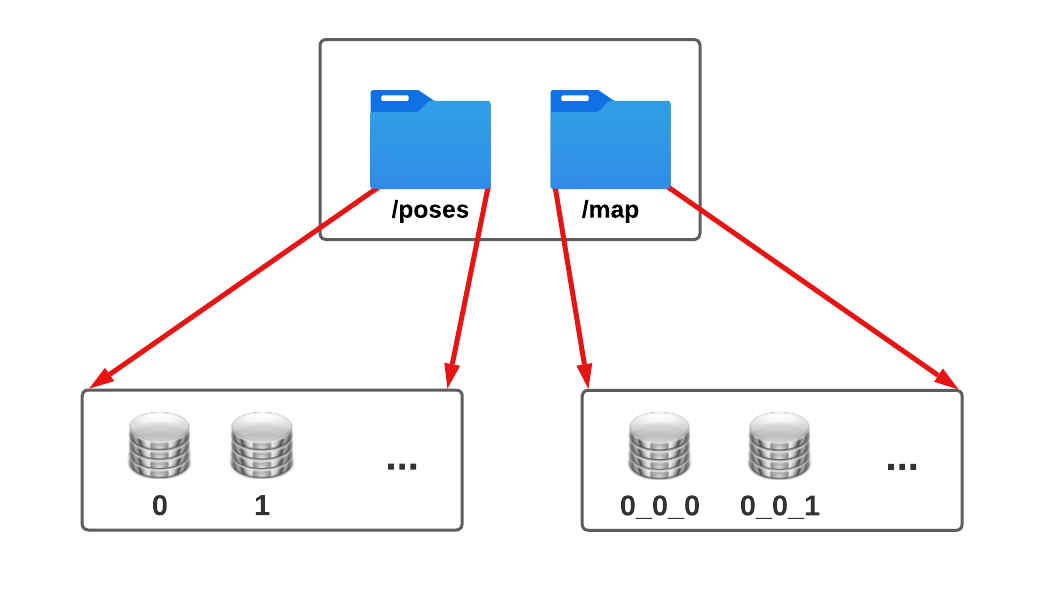
\includegraphics
			[scale=0.25]
			{HDF5old}
		\caption
			[Caption for LOF]{Innere Struktur der HDF5-Datei, die die globale TSDF-Karte repräsentiert. Auf der obersten hierarchischen Ebene werden die Daten in zwei Gruppen aufgeteilt. \emph{/poses} enthält dabei die Trajektorie des Roboters, separiert in einzelne Posen, die mit Null beginnend indiziert sind. \emph{/map} enthält die eigentliche TSDF-Karte. Sie ist in unterteilt in Chunks, die ein Datenarray aus Paaren von TSDF-Wert und TSDF-Gewicht enthalten. Das Label der Chunks entspricht den diskreten Koordinaten der Chunks im Raum.}			                                                                                                                                     
		\label{fig:HDF5old}
\end{figure}

Die Bezeichnung (TSDF-)Karte beziehungsweise \emph{Map} wird im Folgenden für die implizite TSDF Repräsentation der Umgebung verwendet. Der Urpsrung der Karte ist im Folgenden als Ursprung des Weltkoordinatensystems definiert. Der folgende Abschnitt befasst sich mit dem inkrementellen Update der lokalen Karte auf Basis der Daten in Form einer Pose $P_{new}$, deren Translation und Rotation zum Beispiel durch eine Registrierung der zugehörigen Punktwolke $C_{new}$ bestimmt wird. Dieses Update ist nicht mit dem Update der Karte im Anschluss an eine Graph-Optimierung zu verwechseln. Das im folgenden beschriebene Update widmet sich lediglich dem inkrementellen Update der Karte im SLAM und wird getrennt von Schleifenschlüssen und Graph-Optimierungen betrachtet.

\subsection{TSDF-Update}
\label{section:tsdf_update}

Dieser Abschnitt eruiert das inkrementelle Update der lokalen TSDF-Karte basierend auf einer neuen Pose $P_{new}$ und der zugehörigen Scan-Punktwolke $C_{new}$. Dies kann sowohl das erste Datenpaar sein, auf Basis dessen ein Update der TSDF-Karte durchgeführt wird oder ein Datenpaar, welches in eine bereits teilweise befüllte Karten eingefügt wird. Für ein Konsistentes Einfügen der neuen Daten wird dazu die Karte zunächst in Richtung der neuen Pose verschoben, sodass das Zentrum der Karte genau auf der neuen Pose liegt. Dabei werden Teile der lokalen Karte, die außerhalb des neuen Sichtbereichs liegen zurück in die globale Karte geschrieben und Teile der globalen Karte, die nun in den Sichtbereich der lokalen Karte gelangen, aus der globalen Karte nachgeladen. Dieses Verschieben ist optional und kann gegebenenfalls durch andere Strategien ersetzt werden um die Anzahl dieser Laufzeit-intensiven Operationen zu reduzieren. Möglich ist zum Beispiel erst dann eine Verschiebung der Karte durchzuführen, wenn die neue Pose eine definierte Entfernung zum alten Zentrum der Karte überschreitet. Da diese Arbeit den Fokus nicht auf diese Art von Optimierungen legt, wird im Folgenden von einer Verschiebung der Karte für jede neue Pose ausgegangen. Im Anschluss an die Verschiebung ist das neue Zentrum der Karte äquivalent zum Translations-Anteil $t_{new}$ der neuen Pose $P_{new}$. Ausgehend von der Pose werden zum Update der Karte Rays zwischen der neuen Pose und jedem Datenpunkt $p_i$ der Scan-Punktwolke abgelaufen. Der Strahl stoppt dabei nicht am Punkt $p_i$, sondern wird um eine Länge von $\tau$ verlängert, damit auch der negative Bereich bis $-\tau$ berücksichtigt wird. Die vom Strahl $r_i$ geschnittenen TSDF-Zellen der diskretisierten lokalen Karte werden entsprechend der Entfernung des Zentrums der Zelle zum Punkt $p_i$ befüllt. Durch die Diskretisierung der Karte ist es möglich, dass mehrere Strahls dieselbe Zelle schneiden. In diesem Fall wird für die Zelle die kleinste berechnete Distanz gewählt. Die Tupel aus TSDF-Wert und Gewicht $\left\langle \text{value} \left(\upsilon_i \right), \text{weight} \left(\omega_i \right) \right\rangle$ einer vom Strahl $r_i$ in Richtung $p_i$ getroffenen Zelle wird wie folgt berechnet. Dabei bezeichnete $d_i$ die euklidische Distanz des Voxelzentrums zum Punkt $p_i$ \cite{HATSDF, Canelhas2017TruncatedSD}. $d_i$ ist negativ, wenn der Strahl über den Punkt $p_i$ hinaus belaufen wird. Dies ist zunächst nicht der Wert, der in die Karte geschrieben wird, sondern lediglich der, der im späteren Verlauf mit dem aktuellen Karteninhalt verglichen wird und gegebenenfalls für ein Update sorgt.


\begin{myequation}
    \omega_i=
    \begin{cases}
      1 \cdot \frac{(\tau + \upsilon)}{(\tau - \frac{\tau}{10})}, & \text{if}\ \upsilon_i < -\frac{\tau}{10} \\
      1, & \text{otherwise}
    \end{cases}
  \end{myequation}
  
  \begin{myequation}
    \upsilon_i=
    \begin{cases}
     	\min \left( d_i, \tau \right), & \text{if}\ d_i \geq 0 \\
      	\max \left( d_i, -\tau \right), & \text{if}\ d_i < 0 \
    \end{cases}
  \end{myequation}

Diese Gleichungen sind entnommen aus  \cite{HATSDF, Canelhas2017TruncatedSD}. Für das Gewicht ergibt sich eine lineare Abnahme im negativen Bereich, hinter der betrachteten Oberfläche, ab einer gegebenen Schwelle von $\upsilon_{\epsilon} = -\frac{\tau}{10}$. Der TSDF-Wert $\upsilon$ nimmt Werte entsprechend des Intervalls $I_{\upsilon}$, gegeben die Distanz vom Voxel-Zentrum zum Punkt $p_i$, an. Wie zuvor erörtert ist, können mehrere Strahls dieselbe Zelle schneiden. In diesen Fällen wird jeweils das Tupel mit dem TSDF-Wert gewählt, der näher in Richtung der Oberfläche, als einem TSDF-Wert von $0$ gelegen ist. Diese so generierten Tupel werden nun mit dem derzeitigen Inhalt der Karte verglichen. Dabei gelten die folgenden Vorschriften zur Berechnung des in die Karte geschriebenen Tupels $\left\langle  \upsilon_{new}, \omega_{new} \right\rangle$. Gegeben das aktuell in der Karte vorliegende Tupel $\left\langle  \upsilon_{map}, \omega_{map} \right\rangle$, sowie das zuvor berechnete Tupel $\left\langle  \upsilon_{i}, \omega_{i} \right\rangle$. $\omega_{max}$ definiert das maximale Gewicht einer Zelle, welches dafür sorgt das Änderungen an der Zelle, die im späteren Verlauf vorgenommen werden, einen Effekt auf den TSDF-Wert haben können. Es ergibt sich:


  \begin{myequation}
    \omega_{new}=
    \begin{cases}
      \min \left(\omega_{map} + \omega_{i}, \omega_{max} \right), & \text{if}\ \omega_i > 0 \text{ and $\omega_{map} > 0$}  \\
      \omega_i, & \text{if}\ \omega_i \neq 0 \text{ and  $\omega_{map} \leq 0$} 
    \end{cases}
  \end{myequation}
  
  \begin{myequation}
    \upsilon_{new}=
    \begin{cases}
      \frac{\upsilon_{map} \cdot \omega_{map} + \upsilon_{i} \cdot \omega_{i}}{\omega_{map} + \omega_{i}}, & \text{if}\ \omega_i > 0 \text{ and $\omega_{map} > 0$}   \\
      \upsilon_i, & \text{if}\ \omega_i \neq 0 \text{ and  $\omega_{map} \leq 0$}
    \end{cases}
  \end{myequation}

Im Anschluss wird das neue Tupel anstelle der vorliegenden Werte in die Karte geschrieben.
Neben dem Update der vom Strahl geschnittenen Zellen erfolgt zusätzlich eine vertikale Interpolation der umliegenden Zellen aller geschnittenen Zellen \cite{HATSDF}. Diese Idee gründet in den Erfahrungen mit modernen Laserscannern, die ein horizontales Sichtfeld von $360^{\circ}$ aufweisen und in der Horizontalen eine gute Dichte der Punktdaten liefern, allerdings in vertikaler Richtung eine starke Begrenzung der Auflösung durch eine Sensor-spezifische Anzahl von Scan-Linien vorweisen. Die Abstände zwischen den Scan-Linien vergrößern sich dabei mit der Entfernung des Laserscanners zur betrachteten Oberfläche. Dies sorgt für ein dünn besetztes und nicht geschlossenes TSDF mit mehreren Lücken in vertikaler Richtung, abhängig von der Anzahl Scan-Linien des Sensors. Gegeben den Richtungsvektor $\vec{d_{r_i}}$ des Strahls $r_i$, sowie einen Vektor $\vec{up}$, der im lokalen Koordinatensystem des Scanners, gegeben durch die aktuell betrachtete Pose $P_{new}$, in Richtung der z-Achse schaut, ergibt sich der Interpolations-Vektor $\vec{v_{int}}$ als:

\begin{myequation}
\vec{v_{int}} = vec{d_{r_i}} \times \left( vec{d_{r_i}} \times \vec{up} \right)
\end{myequation}

Entlang dieses Vektor wird ausgehend vom aktuellen Schritt $s_i^j$ beim Ablaufen des Strahls $r_i$ eine Interpolation durchgeführt. Die Schrittweite entlang des Strahls ergibt sich aus der Seitenlänge der TSDF-Zellen und wird mit der Hälfte dieser Seitenlänge initialisiert. Es wird sowohl in Richtung $\vec{v_{int}}$ als auch $-\vec{v_{int}}$ interpoliert. Die vom Interpolations-Vektor geschnittenen Zellen erhalten einen identischen TSDF-Wert zu dem der aktuell von $r_i$ geschnittenen Zelle. Dabei werden nur dann Werte in Zellen geschrieben, wenn sie zuvor noch an keiner anderen Stelle beschrieben wurden. Die Interpolation in negative und positive Richtung von $\vec{d_{r_i}}$ ist begrenzt durch den halben Abstand $\Delta_z$ zur nächsten Scan-Linie nach oben und unten und berechnet sich aus dem vertikalen Öffnungswinkel des Sensors $\alpha_{sensor}$ und der Anzahl verfügbarer Scan-Linien $n_{lines}$. Gegeben die Länge des Vektors zwischen der Scanner-Position und dem aktuell betrachteten Schritt $l_s$ als, ergibt sich $\Delta_z$ als:

\begin{myequation}
\Delta_z = \frac{\tan \left( \frac{\alpha_{sensor}}{n_{lines}} \right) \cdot l_s)}{2}
\end{myequation}

Diese Begrenzung sorgt dafür, dass keine Zellen interpoliert werden, die näher an den Strahlen benachbarter Scan-Linien gelegen sind. Damit Zellen, die interpolierte Daten enthalten, identifiziert werden können, wird ein negatives Gewicht zugewiesen. Nicht inkrementelle Updates auf Basis identifizierter Schleifenschlüsse, wie vorgestellt in Kapitel \ref{chapter:association} und \ref{chapter:map_update} müssen die interpolierten Zellen beachten. Im Folgenden wird auf den hier verwendeten SLAM-Ansatz Bezug genommen und die verwendeten Konzepte und Datenstrukturen herausgestellt.

\section{Eingliederung des genutzten SLAM Verfahrens}
\label{section:slam}

Im Stand der Forschung \ref{section:sdf} ist eine Übersicht des SLAM-Forschungsgebiets und eine Erklärung des unterliegenden SLAM-Problems dargelegt. An diese wird nach einer kurzen Rekapitulation mit Fokus auf die Eingliederung des für diesen Ansatz genutzten SLAM-Verfahrens angeknüpft. SLAM ist der Prozess der simultanen Generierung einer Karte einer unbekannten Umgebung und der Lokalisierung innerhalb dieser Karte beziehungsweise Umgebung. SLAM ist ein \emph{Henne-Ei-Problem}, da auf der einen Seite eine vollständige Karte benötigt wird, um die Pose des Roboters akkurat zu bestimmen, auf der anderen Seite allerdings eine akkurate Pose-Historie benötigt wird um eine gute Karte der Umgebung aufbauen zu können. Im Stand der Forschung in Kapitel \ref{section:sdf} ist herausgestellt, dass SLAM Ansätze in der Regel aus der Lokalisierung in einer Karte und dem Prozess der Kartierung zusammengesetzt sind. Im Folgenden wird auf Basis dieser zwei Komponenten der hier verwendete SLAM Ansatz eruiert. Als Grundlage dieser Arbeit dient der SLAM Ansatz von Eisoldt et al. \cite{HATSDF}, der eine implizite, volumetrische TSDF-Darstellung der Oberfläche als Karten-Repräsentation verwendet, die inkrementell erweitert wird. Sowohl die inkrementelle Erweiterung der Karte, als auch die Registrierung neuer Punktdaten über die in \emph{Point-to-TSDF} Strategie stammen aus den Ausführungen von Canelhas \cite{Canelhas2017TruncatedSD}. Zunächst wird der Versuch unternommen auf Basis der Ergebnisse aus \cite{HATSDF} in Form einer TSDF-Karte, die in einer HDF5 gespeichert ist ( siehe \ref{section:tsdf_map}) und der zugehörigen Trajektorie des Roboters eine Optimierung der Trajektorie und ein entsprechendes Update der TSDF-Karte durchzuführen. Im weiteren Verlauf dieser Arbeit wird untersucht, wie Schleifenschlüsse und die daraus resultierende Optimierung des Pose-Graphen und der Karte in den vorliegenden SLAM-Ansatz integriert werden kann, welche Voraussetzungen dafür existieren und wie der hier vorgestellte Ansatz in einer Nachbearbeitung verwendet werden kann. Der folgende Abschnitt stellt die algorithmischen Grundlagen zur Detektion von Schleifenschlüssen heraus und welche Implementationen dafür verwendet werden.

\section{Grundlegende Konzepte für die Identifikation von Schleifenschlüssen}

Der hier verwendete Ansatz zur Identifikation von Schleifenschlüssen basiert auf der \emph{Registrierung} von Punktwolken (siehe Kapitel \ref{chapter:loop_closure}.  Als Registrierung wird der Prozess der Zusammenführung von Punktwolken bezeichnet, die von unterschiedlichen Posen aufgenommen werden. Um Punktwolken möglichst gut zusammenzuführen, wird der Versuch unternommen diese maximal zu überlappen. Dieser Prozess wird auch \emph{Scan-Matching} genannt. Beim Scan-Matching wird zwischen dem \emph{Model} und dem \emph{Scan} unterschieden. Als Scan werden die Daten bezeichnet, die an das Model registriert werden sollen. Das Ergebnis des Scan-Matching ist eine Approximation der Transformation $T_{Scan \rightarrow Model}$ zwischen den Posen die den Punktwolken zugehörig sind. Der dafür in dieser Arbeit verwendete Algorithmus ist der \emph{Generalized Iterative Closest Point (GICP)} Algorithmus nach Segal et al. \cite{segal2009generalized}. Dieser Ansatz basiert auf dem wohlbekannten \emph{Iterative Closest Point (ICP)} Algorithmus zur Registrierung von Punktwolken nach Besl \& McKay \cite{besl1992method}. Sie bestimmen eine Approximation der gesuchten 6-D Transformation zwischen zwei Punktwolken durch die Minimierung der Summe der quadrierten Distanzen der nächsten Punkte zwischen den beiden Punktwolken durch eine \emph{Singular Value Decomposition (SVD)}. Damit untersucht werden kann, wie gut diese Approximation ist, liefern ICP und verwandte Algorithmen wie zum Beispiel GICP ein Maß für die Genauigkeit der Approximation. Dies ist im Fall von ICP und GICP der sogenannte \emph{Fitness-Score}. Er beschreibt die durchschnittliche quadrierte Distanz zwischen den \emph{Nearest-Neighbors (nächsten Nachbarn)} der Punktwolken nach Anwendung der approximierten Transformation $T_{Scan \rightarrow Model}$ zwischen der Scan-Pose und der Model-Pose. Er gibt dementsprechend an, wie groß die durchschnittliche quadrierte Distanz eines Punktes aus der Model-Punktwolke zum euklidisch nächsten Punkt der transformierten Scan-Punktwolke ist. Der GICP-Algorithmus erweitert die von Besl \& McKay \cite{besl1992method} vorgestellten Konzepte um die in \cite{chen1992object} vorgestellte \emph{Point-to-Plane} Metrik und eine \emph{Plane-to-Plane} Metrik. Das Ergebnis dieser Erweiterung ist ein Ansatz zur Registrierung, der die Ergebnisse von ICP im Regelfall sowohl in der Laufzeit, als auch in der Genauigkeit übertrifft \cite{segal2009generalized}. Sowohl ICP, als auch GICP sind inkrementelle Algorithmen, die sich inkrementell einem Optimum immer weiter annähern. Dabei wird die approximierte Transformation jeweils um ein $\delta T$ verändert. Fällt dieses $\delta T$ in einer Iteration unter einen vom Benutzer gewählten Schwellwert, oder wird eine maximale Anzahl an Iterationen erreicht, bricht der jeweilige Algorithmus ab und gibt die finale Transformation zurück. Genanntes Optimum ist dabei im Regelfall allerdings kein globales, sondern lediglich ein lokales Optimum. Aus diesem Grund gilt es die jeweiligen Ausgaben der Algorithmen zu analysieren. Dazu kann zum Beispiel der resultierende Fitness-Score verwendet werden. In dieser Arbeit wird die GICP-Implementation der \emph{Pointcloud-Library (PCL)} \cite{rusu20113d} verwendet. Im folgenden Kapitel wird eine mögliche Nachbearbeitung der Ergebnisse aus \citep{HATSDF} auf Basis der resultierenden TSDF-Karte und zugehörigen Pose-Historie diskutiert.